\documentclass{article}
\usepackage[utf8]{inputenc}
\usepackage{lmodern}
\usepackage{blindtext}
\usepackage{amsmath}
\usepackage[a4paper, inner=1.7cm, outer=2.7cm, top=3cm, bottom=3cm, bindingoffset=1.2cm]{geometry}
\usepackage{tcolorbox}
\usepackage{graphicx}
\usepackage{wrapfig}
\usepackage{makecell}
\usepackage{boldline}
\usepackage{float}
\usepackage{tabularx}

\renewcommand\theadalign{bc}
\renewcommand\theadfont{\bfseries}
\renewcommand\theadgape{\Gape[4pt]}
\renewcommand\cellgape{\Gape[4pt]}

\begin{document}

\title{\textbf{Liquity: Decentralized Borrowing Protocol}}
\author{Robert Lauko, Richard Pardoe \\ rev.0.2\footnote{Note that this white paper is released prior to the full implementation and launch of the project. It is therefore subject to correction, completion and amendment without notice}\footnote{Note as well that whenever the term Liquity is used it refers to the protocol, not the company Liquity AG.}}
\date{February 10, 2021}

\maketitle

\section*{Abstract}
Liquity is a decentralized protocol that allows Ether holders to obtain maximum liquidity against their collateral without paying interest. After locking up ETH as collateral in a smart contract and creating an individual position called a “Trove”, the user can get instant liquidity by minting LUSD, a USD-pegged stablecoin. Each Trove is required to be collateralized at a minimum of 110\%. Any owner of LUSD can redeem their stablecoins for the underlying collateral at any time. The redemption mechanism along with algorithmically adjusted fees guarantee a minimum stablecoin value of \$1. 

An unprecedented liquidation mechanism based on incentivized stability deposits and a redistribution cycle from riskier to safer Troves provides stability at a much lower collateral ratio than current systems. Stability is maintained via economically-driven user interactions and arbitrage, rather than by active governance or monetary interventions. 
The protocol has built-in incentives that encourage both early adoption and the operation of multiple front ends, enhancing decentralization.

\newpage

\tableofcontents

\section{Introduction and competitive landscape}

\subsection{Stablecoins and collateralized debt platforms}
Cryptocurrencies such as Bitcoin or Ether have shown significantly higher price volatility than traditional asset classes like stocks or bonds. Nevertheless, many people use tokens for investments, payments, trading or pure speculation.

Fiat-backed stablecoins like Tether, USDC, Paxos and TrueUSD have emerged as a stable, but centralized alternative to volatile tokens. Additionally, crypto-backed stablecoins have become increasingly popular and a fundamental driver for the Decentralized Finance (DeFi) movement. Acting as collateralized debt platforms, MakerDAO, Equilibrium and Synthetix allow holders to lock up volatile tokens in exchange for freshly generated stablecoins. Owners can thus unlock some of the economic value of their tokens while remaining fully invested. Beyond that, token holders can achieve leverage by using the obtained liquidity to lock up additional collateral to get even more liquidity.
\subsection{Shortcomings of collateralized debt platforms}
Collateralized debt platforms do not rely on lenders to provide liquidity as they can mint the stablecoins themselves. With no refinancing costs, such systems can generate liquidity for free. Yet, most platforms charge recurring fees for borrowing (as high as 20.5\% p.a\footnote{Stability fee charged by MakerDAO in summer 2019}) which accumulate over time. The variable fees (stability fees) are meant to regulate coin supply in order to maintain the peg of the issued stablecoin, and correspond to an interest rate in traditional banking. Affecting new and existing loans alike, interest rates only have an indirect impact on monetary supply and are rather ineffective in the short term. While existing borrowers may not have the means to repay their loans as an immediate reaction to rising interest, short-term speculators and leverage seekers might not be greatly affected by interest rates in the first place.

Often times, governance token holders are expected to manage the economic parameters of their systems (e.g. set the fee rate) in the best interest of the protocol. In practice, on-chain governance has been a difficult and heavily debated topic, with notoriously low turnouts, potentially misaligned incentives, and a high concentration of power in the hands of a few.

In addition to charging stability fees, existing platforms typically require the individual borrower’s position to be significantly overcollateralized\footnote{130\% (Equilibrium, MakerDAO ETH-B), 150\% (MakerDAO ETH-A), or even 750\% (Synthetix).}. This makes the positions capital inefficient since borrowers tend to maintain much higher collateral ratios in practice than the minimum\footnote{The overall total ratio of MakerDAO and Equilibrium is usually between 250\% and 500\%.}. Existing platforms require overcollateralization due to the liquidation mechanisms they apply to positions that become undercollateralized. Both collateral auctions and fixed-price selloffs have turned out to be inefficient by design, leaving room for improvement.

Finally, crypto-backed stablecoins are not generally redeemable at face value and cannot guarantee a hard price peg due to the lack of direct arbitrage cycles\footnote{See https://medium.com/@hasufly/maker-dai-stable-but-not-scalable-3107ba730484.}. There is no issuance or redemption mechanism that would enable arbitrageurs to make guaranteed profits by buying freshly minted stablecoins or selling them back to the protocol whenever the price deviates from the peg. Instead, the systems rely on a less effective soft peg mechanism, which stabilizes the exchange rate by making the loans more or less attractive through variable fees. Crypto-backed stablecoins are thus usually subject to higher price volatility than fiat-backed stablecoins.\\

To summarize, existing collateralized debt platforms have the following downsides:
\begin{itemize}
    \item High and unpredictable interest fees for borrowers
    \item Problematic governance mechanisms
    \item Necessarily high collateralization ratios, due to inefficient liquidation processes
    \item No direct redemption mechanism to ensure price stability
\end{itemize}
 
\section{Key benefits of the Liquity protocol}
A better system is possible. Liquity improves upon the mentioned issues by offering the following key benefits:
\begin{itemize}
    \item Interest-free liquidity
    \item Low collateralization ratio (110\%)
    \item Hard price floor
    \item Governance-free algorithmic monetary policy
    \item Censorship resistance
    \item Growth incentives
\end{itemize}

\subsection{Interest-free liquidity}
Liquity provides liquidity without charging borrowers interest or recurring fees. ETH holders can obtain liquidity against their collateral for free. However, as an algorithmically controlled monetary instrument, the protocol charges an issuance fee (as a one-time fee) for newly drawn liquidity to support the peg with the USD.

Users are free to utilize their stablecoin, LUSD, to participate in the broader DeFi market consisting of many different products which are designed to generate yield.

\subsection{Low collateralization ratio (110\%)}
When an individual position’s collateral ratio falls below a certain threshold, a lending system must take special action to ensure the stablecoin supply remains fully backed. In existing systems, this is done by liquidating the position in an interactive process. Selling the collateral from undercollateralized positions at a fixed price is inefficient by design as it requires a significant discount to the current collateral price to ensure that it can be sold quickly in difficult situations. Collateral auctions replace discounts by an economically fair, but potentially lengthy and error-prone\footnote{On March 12 (“Black Thursday”) and 13, 2020, 35 000 ETH worth \$8.32 million were withdrawn through zero bids in MakerDAO’s collateral auctions due to the dramatic increase of the Ethereum gas price. See https://medium.com/@whiterabbit/black-thursday-for-makerdao-8-32-million-was-liquidated-for-0-dai-36b83cac56b6} bidding mechanism. The longer it takes to sell the collateral\footnote{The duration of the auction usually depends on the number of bidders, which creates an unfortunate tradeoff since a large number of bidders is good for the auction, but potentially leads to longer auctions and higher exogenous price risks.}, the higher the risk that its value might drop further. Auction-based systems thus have to set their liquidation ratio\footnote{The ratio between the current collateral value (in USD) and the debt below which a liquidation may occur. The liquidation ratio may or may not equal the minimum collateral ratio needed to open a position.} high enough to provide an extra margin for subsequent price drops during liquidation.

Liquity applies a novel two-step liquidation mechanism aimed at instantly liquidating undercollateralized positions. Since the acquirers are known in advance, there is no need to find a buyer for a collateral buyout on the spot when a position becomes undercollateralized. This advantage allows for a considerable reduction in the collateralization ratio, while keeping stability high. The system also relies on sufficient collateralization of all positions in aggregate, rather than on the collateral of individual positions.

\subsection{Hard price floor}
Liquity follows a maximally expansive monetary policy through providing free liquidity at zero issuance costs by default. On the other hand, the issued LUSD tokens are fully redeemable against the collateral. This enables the protocol to grow rapidly, but not so fast as to lose control over the peg.

LUSD tokens can be returned to the protocol (redeemed) in exchange for an ETH amount worth the face value of the returned LUSD minus a redemption fee. This direct price stability mechanism results in a price floor of \$1. At lower rates, arbitrageurs can make profits by redeeming LUSD for ETH and immediately selling the latter at a higher dollar price than the current value of the returned LUSD. Arbitrageurs will thus help to restore the peg by driving demand for LUSD, as the redemption fees are designed to enable arbitrage gains whenever the peg is broken.

\subsection{Governance-free algorithmic monetary policy}
Unlike competing platforms, Liquity does not rely on a governance mechanism to vote on monetary interventions like changing an interest rate. All protocol parameters are either preset and immutable or algorithmically controlled by the protocol itself, making governance redundant.

Liquity uses the current fraction of redeemed LUSD as an indicator of a peg deviation in order to autonomously set a base rate, which determines both the redemption fee and the issuance fee. The base rate increases with the number of redeemed tokens and tends to decay to 0\% again when no redemptions take place. As opposed to an unpredictably fluctuating interest-rate, the issuance fee immediately and predictably reduces the attractiveness of new loans and throttles the generation of fresh LUSD. In addition, redemption of LUSD for ETH directly decreases the current stablecoin supply and may motivate low-collateral borrowers to repay their loans, which has the same effect. 

These measures exert upward pressure on the value of LUSD whenever it is less than \$1, and help to stabilize its price.

\subsection{Censorship resistance}
Liquity is a protocol rather than a platform. There is no administrator with special privileges that could interfere with, alter, or halt the operation of the protocol in any way.

Frontend operation is provided by third parties which make the system decentralized and resistant to censorship, while benefiting from growth incentives. Frontend Operators can either download the web interface provided as a launch kit or opt for creating their own custom user interface and integrate it with other services.

\subsection{Growth and early adopter incentives}
Users that drive growth and robustness by contributing to system stability get rewarded with LQTY, the system's secondary token. These tokens can be staked in order to earn a proportion of the protocol revenue stemming from issuance and redemption fees. The protocol continuously issues LQTY to front ends and to users who have deposited LUSD to the Stability Pool. LQTY is issued according to a release schedule that halves the number of tokens distributed each year, favoring early adopters.

The allocation of LQTY between Frontend Operators and users is based on a kickback rate that can be freely set by the front end operator between 0\% and 100\%. Front ends will thus compete via the kickback rates, making the system attractive to users and early adopters.

\section{System functionality}
\subsection{Borrower operations }
Anyone may obtain liquidity anytime in an entirely permissionless manner after depositing ETH into a \textbf{Trove\footnote{Each Trove is linked to a specific Ethereum address. An Ethereum address can only own one single Trove.} }.The deposited ETH collateral gets locked up in the Trove and allows its owner to withdraw up to \textbf{90.91\%}\footnote{Called loan-to-value ratio or LTV.} of its current dollar value in the form of LUSD stablecoins. In other words, the Trove must always maintain a \textbf{minimum collateral ratio (MCR)} of 110\%, defined as the ratio of the current dollar value of the collateral to the withdrawn liquidity. Borrowers can repay or borrow more liquidity within the limits of the MCR whenever they wish. Within the same limit, they can retrieve their collateral. Moreover, a Trove can be topped up with more collateral as needed. \\

\textit{Liquidation Reserve}. When a borrower opens a new Trove, an amount of 50 LUSD is reserved and held back by the protocol as a compensation for the gas costs if the Trove needs to be liquidated at some point. The 50 LUSD is added to the Trove's debt, leading to a minimum collateral requirement of 55 USD worth of ETH\footnote{This requirement also makes it harder to spam the system by creating very small Troves.}. When a borrower closes their Trove, the Liquidation Reserve is refunded, i.e. the corresponding 50 LUSD debt on the Trove is cancelled. The borrower thus needs to pay back 50 LUSD less to fully pay off their debt. \\

\textit{Issuance fee}.   The protocol charges a one-time issuance fee for the borrowed liquidity. The fee is added to the Trove's debt and is given by a \textbf{base rate} (see 3.3 Redemption mechanism “Redemption fee and base rate”) multiplied by the amount of liquidity drawn by the borrower. The minimum issuance fee is 0.5\%, and the maximum is 5\%. \\

\begin{tcolorbox}
\textbf{Example}\\
The base rate stands at 1.2\%. The borrower opens a new Trove by depositing 5 ETH and draws 1,000 LUSD. Being subject to a Liquidation Reserve of 50 LUSD and charged a 1.2\% fee on the 1,000 LUSD, the borrower will obtain 1,000 LUSD, but their initial debt will be set to 1,062 (1,000 + 50 + 12) LUSD. To close the Trove and fully retrieve the 5 ETH, the borrower needs to repay 1,012 LUSD as the Liquidation Reserve gets refunded.
\end{tcolorbox}

\textit{Restrictions due to Recovery Mode}.   Borrower operations are restricted in several respects when the system is in Recovery Mode or at the verge of it (see 5 Recovery Mode). 

To avoid liquidation despite ETH price changes, it is highly recommended to keep the collateral ratio of a Trove well above the MCR. Given that in Recovery Mode, liquidations may even affect Troves with higher collateral ratios (maximally up to 150\%), risk averse borrowers should sufficiently collateralize their Troves to avoid being near the bottom tiers of collateralization relative to other Troves whenever the system is close to Recovery Mode. Maintaining a relatively high collateral ratio high also reduces the risk of getting hit by a redemption (see 3.3 Redemption mechanism).

\subsection{Stability Pool operations}
The Stability Pool is the first line of defense in maintaining system solvency: stability deposits absorb and cancel the debt from defaulted Troves. In return, Stability Pool participants are rewarded with the acquisition of collateral from liquidated positions at a significant discount. Participants will also continuously receive an allocation of LQTY tokens.
LUSD holders can become Stability Providers by depositing LUSD tokens into the Stability Pool. In principle, the deposited tokens can be withdrawn from the pool anytime, so long as they have not been used for absorbing defaulted Troves. However, deposit withdrawal is temporarily disabled when there are undercollateralized Troves in the system that can be liquidated.

When a Trove is liquidated, some amount of LUSD in the Stability Pool which corresponds to the debt of the liquidated Trove is burned. In exchange, the Stability Pool receives all of the collateral from that Trove. Because liquidations happen just below 110\%, this means participants achieve a collateral gain in ETH at the time of liquidation. The Stability Providers’s current deposit as a proportion of the total LUSD in the pool determines the collateral share it receives from the liquidation\footnote{As a deposit will shrink over time by absorbing liquidations, the reward calculation results in a “negative” compounding of the deposited LUSD.}. 

While Stability Providers are free to withdraw all or part of their remaining LUSD deposit, the system always pays out the entire collateral gain made by the depositor. Stability Providers that are also borrowers can choose to transfer the collateral gain to their Troves instead of paying it out to their Ethereum addresses. In other words, the system uses the accumulated ETH to top up their own collateral. 

\subsection{Redemption mechanism}
Liquity’s token, LUSD, is a fully redeemable stablecoin. At any time\footnote{To protect the system from bank run-like situations, redemptions are suspended if the total collateralization ratio (TCR) is below 110\%.}, the system allows holders to redeem their LUSD tokens for the underlying ETH collateral based on the face value of the redeemed tokens, the current ETH:USD rate and the current base rate. This enables direct arbitrage whenever LUSD trades for less than \$1, by creating a \textbf{price floor for LUSD}.\\

\begin{figure}[h]
\centering
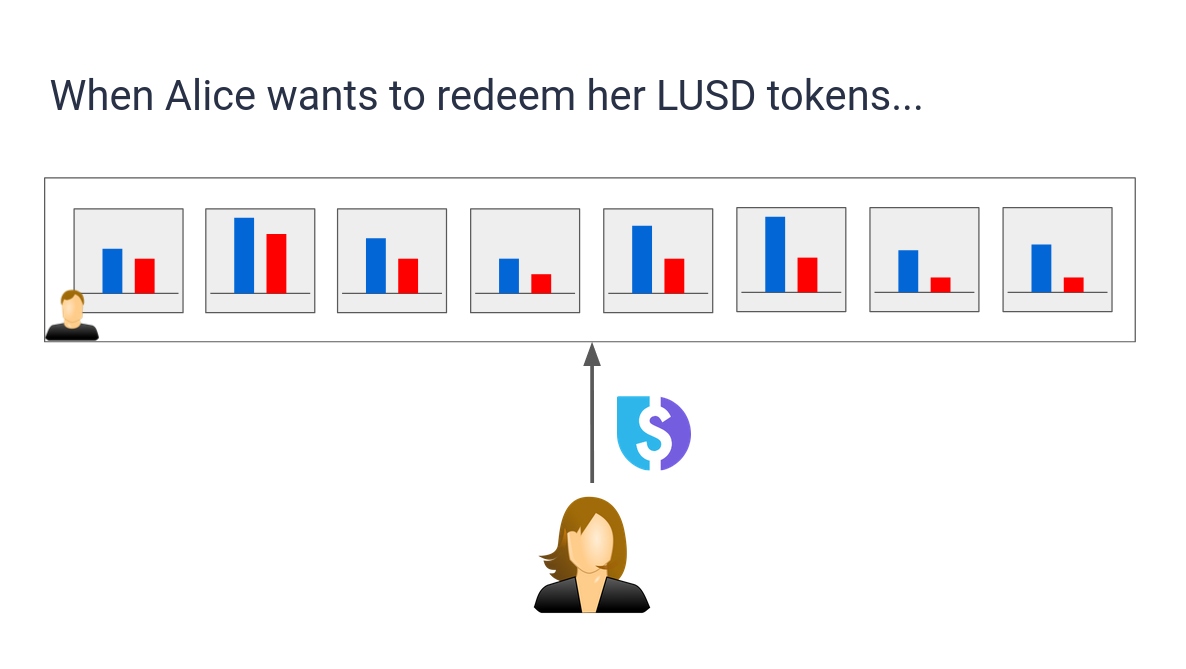
\includegraphics[width=6.75cm]{a1.png}
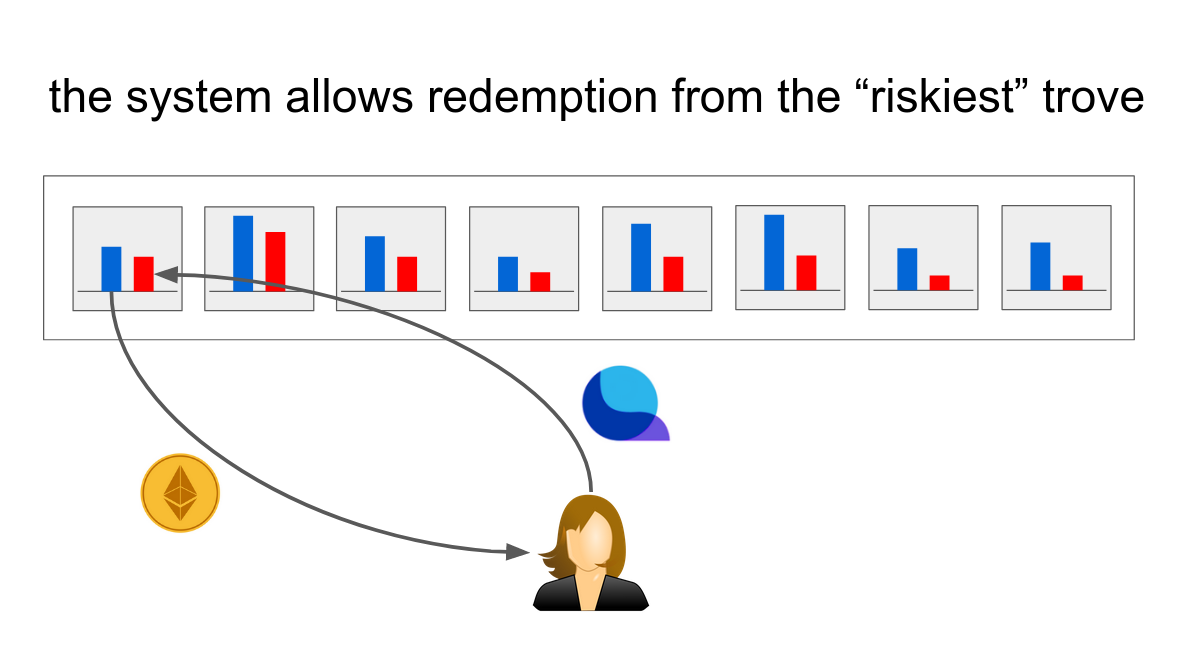
\includegraphics[width=6.75cm]{a2.png}
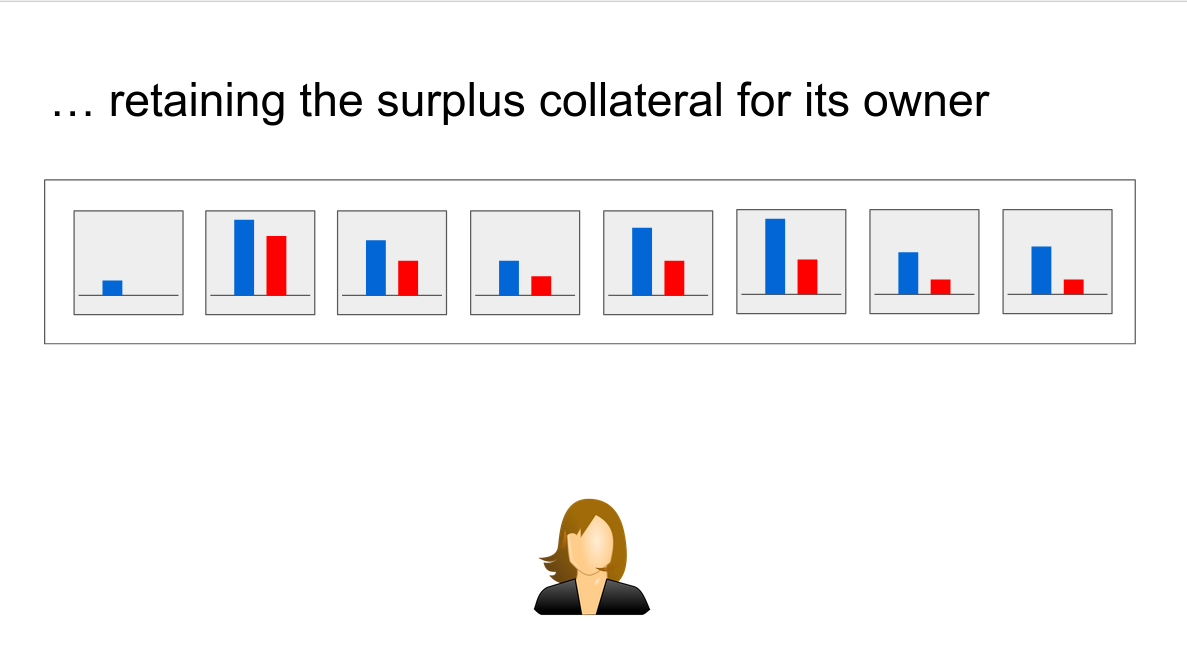
\includegraphics[width=6.75cm]{a3.png}
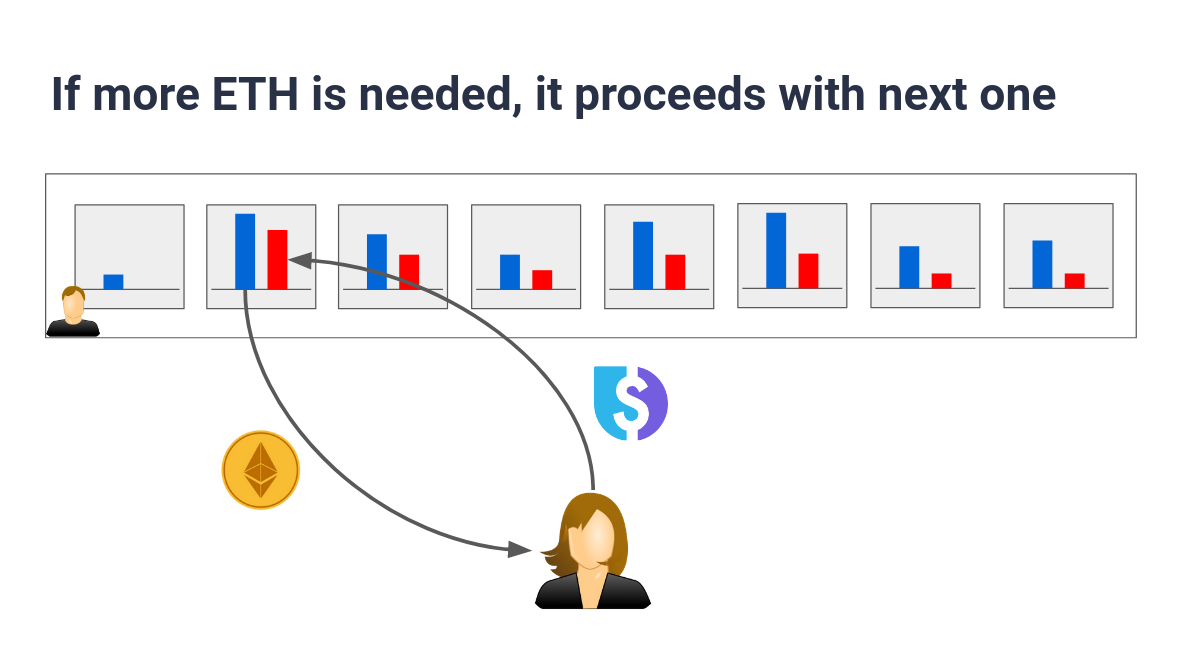
\includegraphics[width=6.75cm]{a4.png}
\end{figure}

When redeemed, the system uses the LUSD to repay the riskiest Trove(s) with the currently lowest collateral ratio, and transfers the respective amount of ETH from the affected positions to the redeemer. The amount taken from each borrower is capped by their corresponding debt, so the affected borrowers can keep their collateral surpluses. In other words, borrowers lose the same nominal amount of debt (in LUSD) as they lose collateral (in USD) and do not suffer a net loss from redemptions. On the flipside, redemptions have a positive effect on the total collateralization of the system, increasing robustness and price stability.

Troves that are fully redeemed from, i.e. whose debt is 0, are automatically closed, and the borrower can reclaim the ETH surplus.\\

\textit{Redemption fee and base rate}. Liquity aims to determine the redemption fee in function of the current base rate and the redeemed LUSD amount as a proportion of the entire stablecoin supply. The base rate is initialized to 0\% at system launch.

Upon every redemption, the base rate is increased by the proportion of redeemed LUSD and then applied to the current redemption as follows:
$$b(t):=b(t-1)+\alpha\times\frac{m}{n}$$
where $b(t)$ is the base rate at time $t,m$ the amount of redeemed LUSD, $n$ the current supply of LUSD and $\alpha$ a constant parameter.\\

The base rate decays over time due to a decay factor that is applied with every redemption and issuance of LUSD prior to calculating the resulting fee. The decay is of the form:
$$b(t):=b(t-1)\times\delta^{\triangle t}$$
where $\delta$ is a decay factor (e.g. 0.94) and $\triangle t$ the time elapsed since the last redemption or loan issuance. The decay factor $\delta$ is chosen such that the half-life of the base rate is 12 hours. \\

Redemptions are thus subject to a \textbf{redemption fee} which is a function of the \textbf{base rate} and the redeemed amount of LUSD. The minimum redemption fee is 0.5\%. The fee is subtracted from the redeemed LUSD, reducing the ETH that the redeemer receives in return.\\
\begin{tcolorbox}
\textbf{Example}\\
LUSD currently trades at \$0.95, and the current base rate is 1.4\%. An arbitrageur redeems 150,000 LUSD, while the total LUSD supply is 10 million. The last redemption happened 2 hours ago and no liquidity has been issued in the meantime. The hourly decay factor is 0.94.\\

The system first applies the decay rate to the current base rate:
$$b(t):=b(t-1)\times\delta^{\triangle t}=0.014\times0.94^2=0.01237$$
It then increases the base rate given the redeemed amount ($\alpha= 0.5$):
$$b(t):=b(t-1)+0.5\times\frac{m}{n}=0.01237+0.5\times\frac{150000}{10000000}=0.01987$$
\\

As a result, the redeemer receives 147,019.44 USD [$150,000 \times (1 - 0.01987)$] worth of ETH. Since the exchanged LUSD is currently worth only 142,500 USD [$150,000 \times 0.95$], the redeemer achieves an arbitrage gain of USD 4,519.44.
\end{tcolorbox}

\section{Trove liquidation mechanism}
To ensure that the entire stablecoin supply remains fully backed by collateral, Troves that fall under the minimum collateral ratio of 110\% (referred to as “undercollateralized”) are subject to liquidation.

Liquidation can be triggered by anybody and allows liquidating multiple Troves in one batch, either by specifying a set of Troves or in ascending order starting from the Trove with the lowest collateral ratio. While the former approach allows to quickly liquidate large Troves, the latter is more resilient against the race conditions that may occur in case of multiple simultaneous liquidations.

In most cases, Stability Providers and/or high-collateral Troves will have a financial incentive to trigger liquidations as fast as possible. To compensate for the gas costs of a liquidation even in times with high prices, Liquity pays the reserved 50 LUSD (see 3.1 Borrower operations) plus 0.5\% of the Trove’s collateral (ETH) to the liquidator.
\\

Liquity utilizes a two-step liquidation mechanism in the following order of priority:
\begin{enumerate}
    \item Offset undercollateralized Troves against the Stability Pool
    \item Redistribute undercollateralized Troves to other borrowers
\end{enumerate}

\subsection{Offset undercollateralized Troves against the Stability Pool}
As mentioned above, the Stability Pool is funded by Stability Providers who deposit LUSD tokens to the contract. It primarily functions as a “shock absorber”: deposited tokens soak up liquidated LUSD debts, and depositors are rewarded for their contribution. 

When a Trove becomes undercollateralized ($<$110\%) due to a drop in the ETH price, the debt (in LUSD) can be immediately offset against the same amount of pooled LUSD tokens, which get burned by the system. In return, the system transfers 99.5\% of the collateral (in ETH) from the liquidated Trove to the Stability Pool, while paying out the remaining 0.5\% to the liquidator.\\

\begin{figure}[h]
\centering
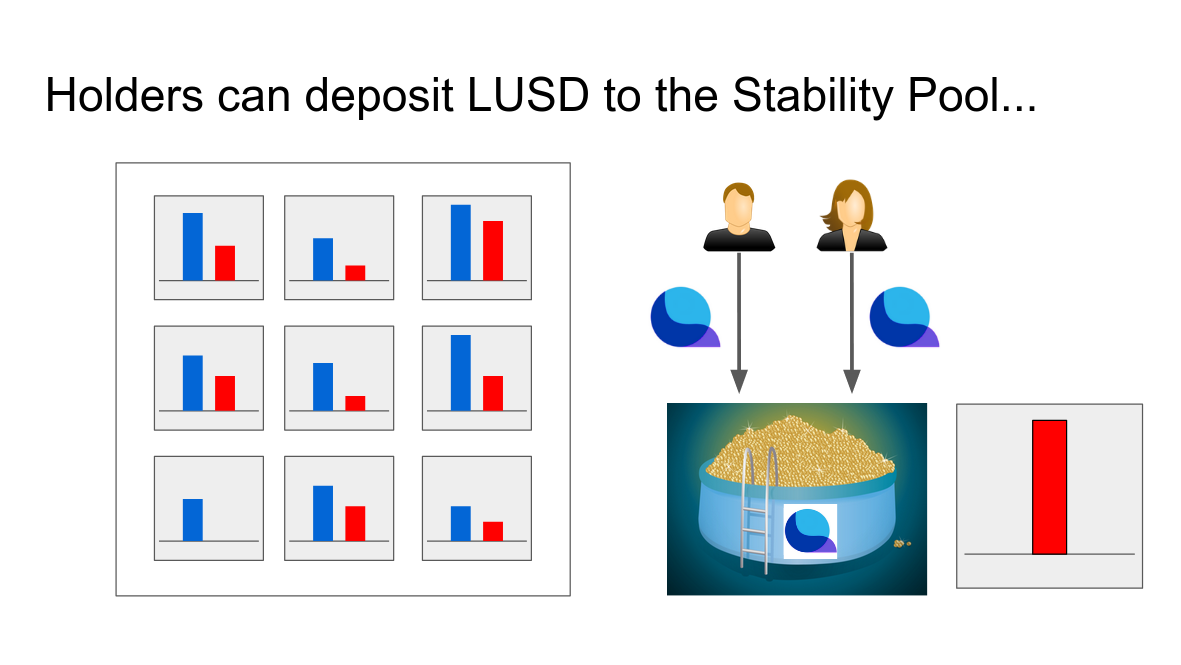
\includegraphics[width=6.75cm]{a5.png}
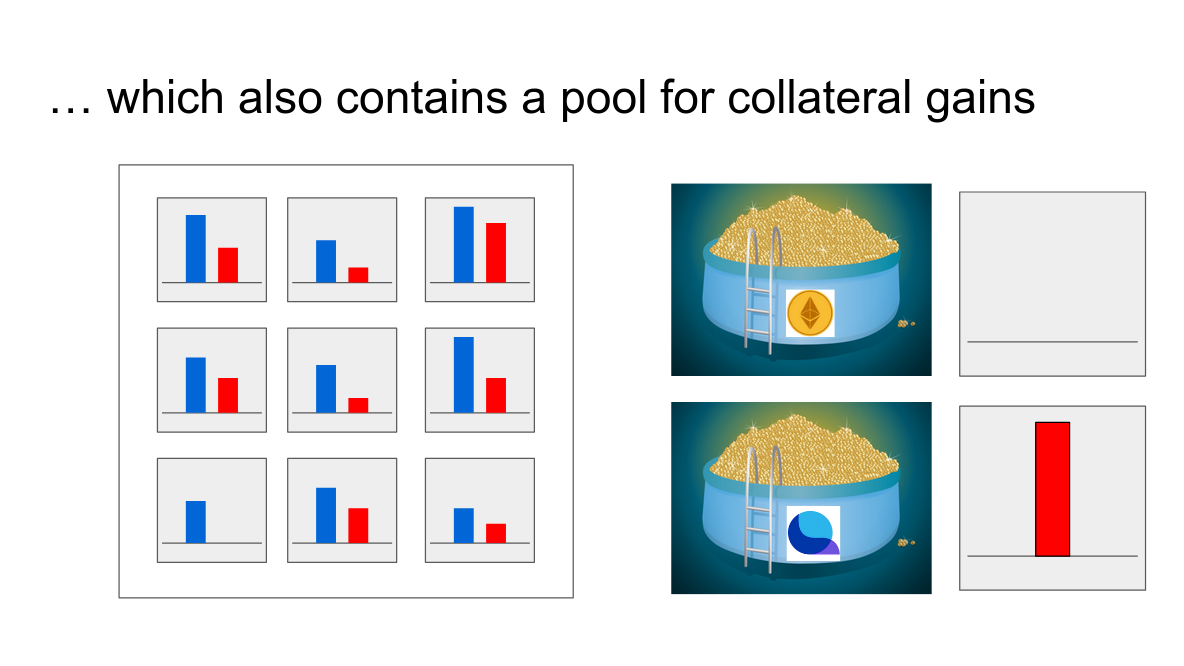
\includegraphics[width=6.75cm]{a6.png}
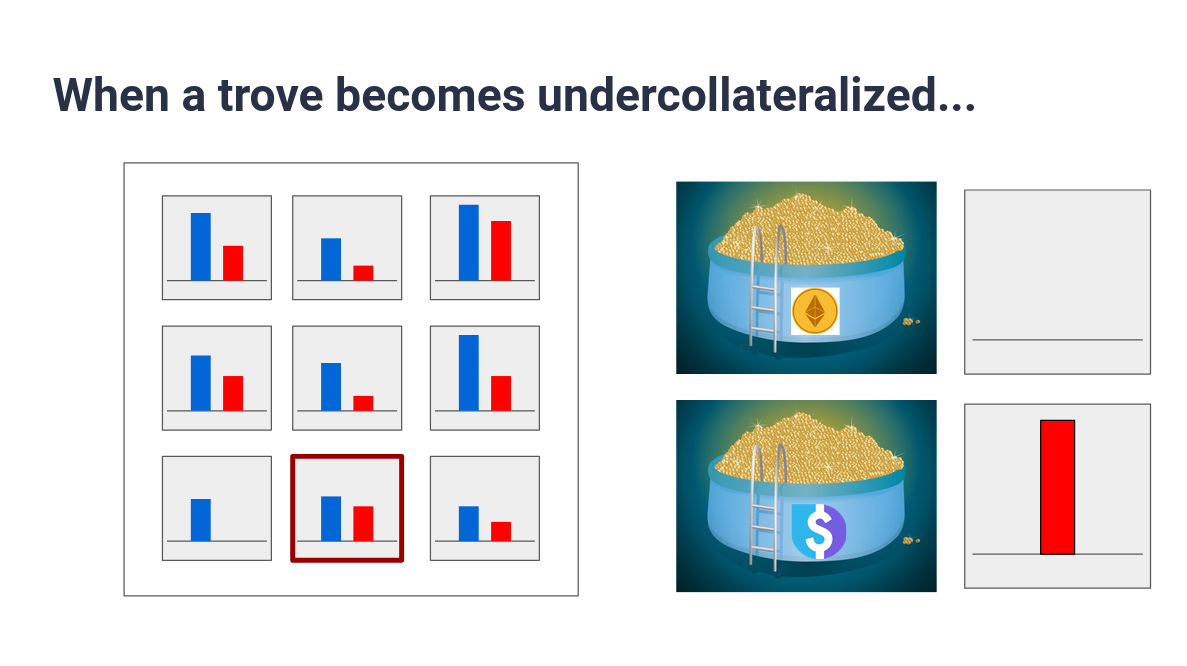
\includegraphics[width=6.75cm]{a7.png}
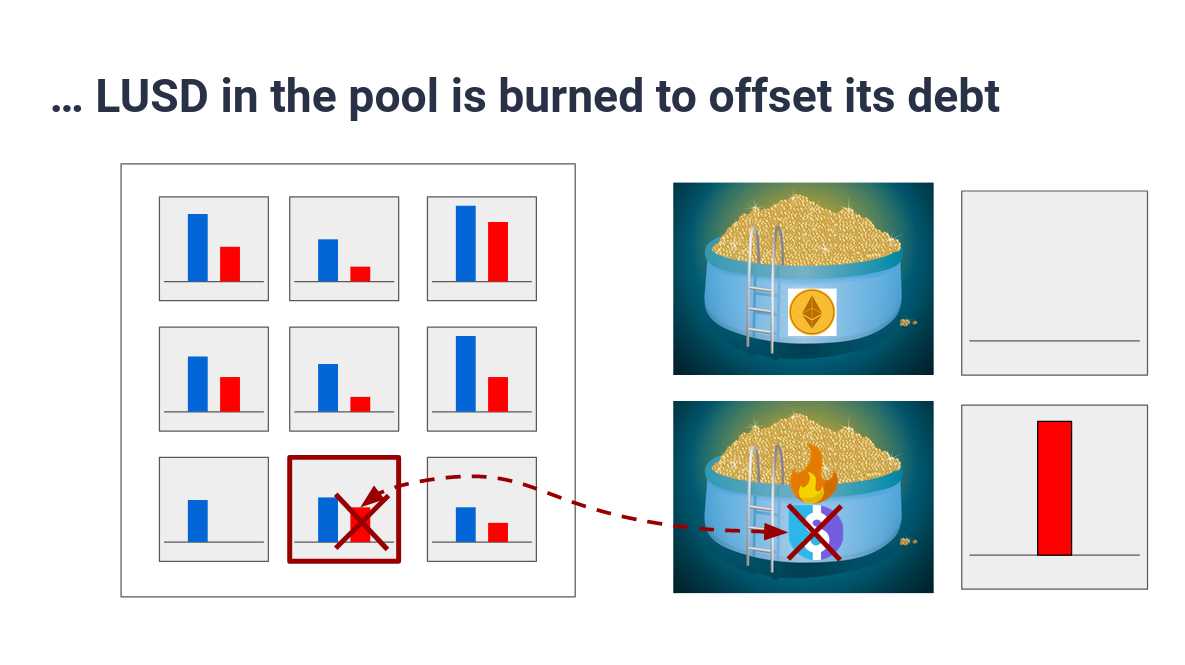
\includegraphics[width=6.75cm]{a8.png}
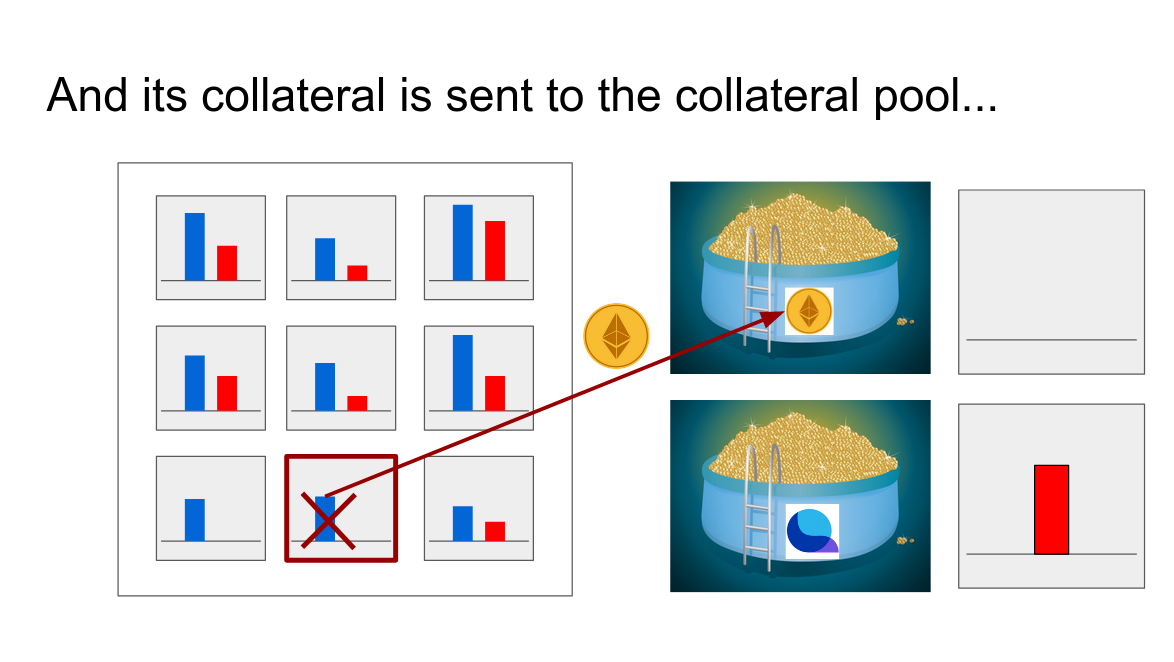
\includegraphics[width=6.75cm]{a9.png}
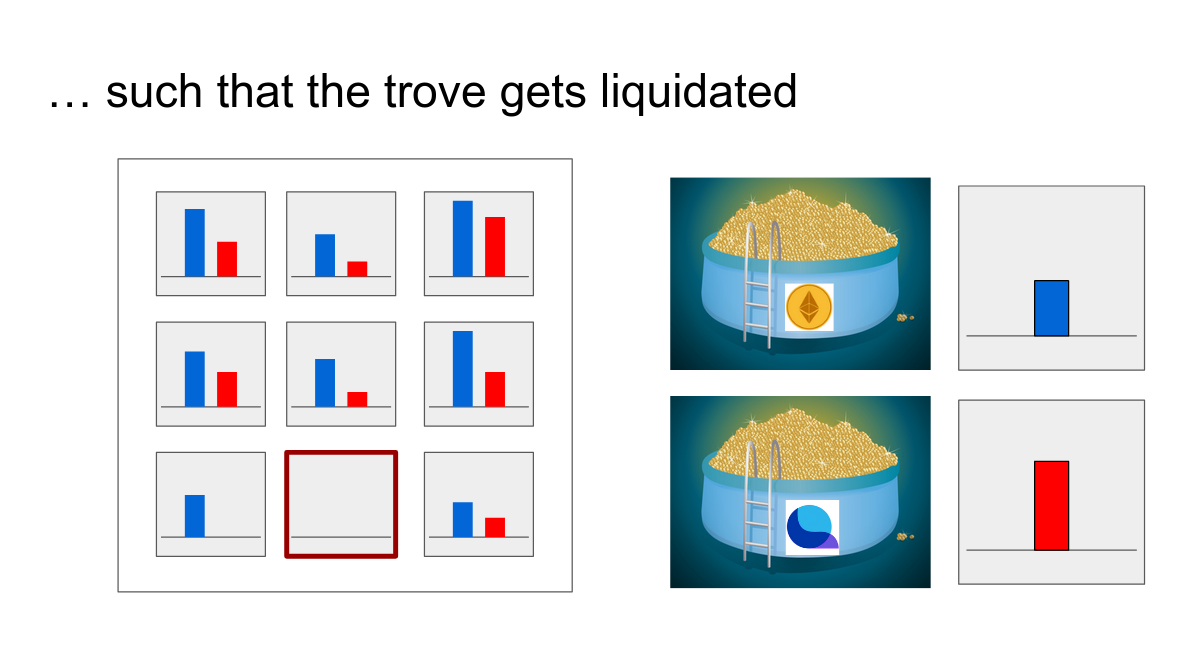
\includegraphics[width=6.75cm]{a10.png}
\end{figure}

The LUSD tokens in the Stability Pool will thus be replaced by ETH over time. Generally, each liquidation contributes a \textbf{collateral surplus gain} to the pool: the collateral is almost always worth more (in USD) than the burned LUSD tokens. This holds because the liquidation is triggered below a collateral ratio of 110\%, but with a very high probability significantly above 100\%\footnote{The actual liquidation ratio depends on the price volatility and the update frequency of the price oracle and will be slightly lower than 110\%. Liquity uses the Chainlink oracle which updates the ETH:USD price every 3 hours and whenever the price changes by more than 0.5\%.} (unless ETH drops by $>$9.09\% between two price feed updates).

A Stability Provider receives shares of the liquidations that occur during the lifetime of their LUSD deposit. Upon obtaining the collateral, the combined value of the remaining LUSD deposit and the ETH gain will very likely exceed the prior value of deposit. Stability Providers are thus incentivized by this expectation of positive returns.

An individual’s share of the surplus gains depends on the ratio of its remaining LUSD deposit (as reduced by past liquidations) to the total amount of LUSD contained in the pool. If no new deposits are made, all individual shares will stay the same throughout liquidations. As new deposits are made, earlier depositors are incentivized to top up their deposit, to maintain their share of future rewards.

\subsection{Redistribute undercollateralized Troves to other borrowers}
It is possible that the LUSD tokens contained in the Stability Pool are not sufficient to offset all undercollateralized Troves, or that a trove’s debt can only be partially absorbed as the Stability Pool runs out of LUSD during a liquidation. In such a case, the system redistributes the remaining debt and collateral from the partially liquidated Trove as well as the remaining undercollateralized Troves to all existing positions.

The redistribution of the collateral and debt is done in proportion to the recipient Trove’s collateral amount. This means that Troves which are heavily collateralized will receive more debt and collateral from liquidated positions than those with low collateralization, ensuring that the system does not create cascading liquidations.\\

\begin{tcolorbox}
\textbf{Example}\\
The two charts show the Troves A, B, C and D with their debt and collateral amounts. Trove D has become undercollateralized and is redistributed to A, B and C.
\end{tcolorbox}

\renewcommand{\arraystretch}{1.3}
\begin{table}[hbt!]
  \small
  \begin{center}
    \caption{Trove debt and collateral amounts.}
    \label{tab:table1}
    \begin{tabular}{|m{0.053\textwidth}|m{0.045\textwidth}|m{0.06\textwidth}|m{0.044\textwidth}|m{0.08\textwidth}|m{0.08\textwidth}|m{0.068\textwidth}|m{0.087\textwidth}|m{0.1\textwidth}|m{0.1\textwidth}|}
    \hline
    \thead{Trove} & \thead{Debt} & \thead{Coll. \\ ETH} & \thead{CR} & \thead{Debt \\ increase} & \thead{Coll. \\ increase} & \thead{New \\ debt} & \thead{New coll. \\ ETH} & \thead{New CR} & \thead{Net gain \\ USD} \\
     \hline
      A & $1000$ & $10$ & $200\%$ & $400.00$ & $2.15$ & $1400.00$ & $12.15$ & $174\%$ & $30$ \\
     \hline
      B & $2000$ & $30$ & $300\%$ & $1200.00$ & $6.45$ & $3200.00$ & $36.45$ & $228\%$ & $90$ \\
     \hline
      C & $3000$ & $60$ & $400\%$ & $2400.00$ & $12.90$ & $5400.00$ & $72.90$ & $270\%$ & $180$ \\
     \hline
      D & $4000$ & $21.5$ & $108\%$ & $-4000.00$ & $-21.50$ & $0.00$ & $0.00$ & n/a & $-300$ \\
     \hlineB{2.5}
      Total & $10000$ & $121.5$ & $243\%$ & $0.00$ & $0.00$ & $10000.00$ & $121.50$ & $243\%$ & $0.00$ \\
      \hline
    \end{tabular}
  \end{center}
\end{table}

\begin{figure}[H]
\centering
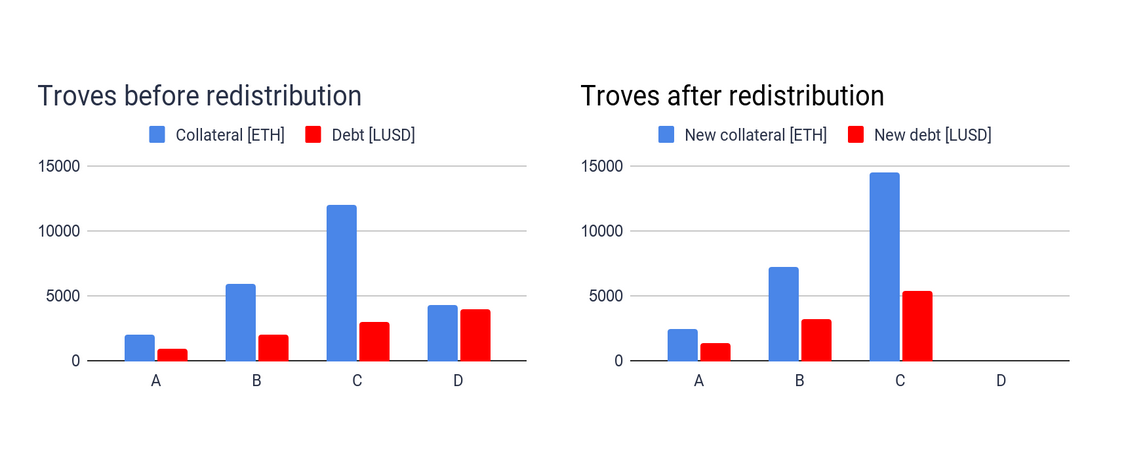
\includegraphics[width=16cm]{a12.png}
\end{figure} 

Receiving collateral and debt shares should generally result in a \textbf{net gain for borrowers}, though at the same time it reduces their own collateral ratios. The risk of being drawn down and becoming undercollateralized as a recipient is minimal, and only affects Troves that are already very close to the minimum collateral ratio (e.g. 111\%).

\section{Recovery mode}
System solvency depends on the amount of LUSD tokens in the Stability Pool and ultimately on the total collateral ratio (TCR) across all Troves, given by the total collateral (in USD) divided by the total debt (in LUSD). 

To keep the system sufficiently collateralized even in times of crisis, the protocol incorporates a Recovery Mode, which is triggered as an \textbf{ultima ratio} if the TCR falls below the critical collateral ratio (CCR) which is set to 150\%. In this special mode of operation, Troves with a collateral ratio between 110\% and the current TCR become subject to liquidation as well. Such extra liquidations are only possible against the Stability Pool (i.e. they are exempt from redistribution), and require that the entire debt can be liquidated at once. 

To protect the borrower from an excessive loss, the collateral that is offset against the Stability Pool is capped at 110\% of the liquidated debt. The borrower can reclaim any collateral remainder above 110\% any time after the liquidation.

During Recovery Mode, the liquidation mechanism is thus described by the following rules:\\

\begin{table}[hbt!]
  \begin{center}
    \caption{Recovery Mode.}
    \label{tab:table1}
    \begin{tabular}{l|l} % <-- Alignments: 1st column left, 2nd middle and 3rd right, with vertical lines in between
      \textbf{Trove's Collateral Ratio} & \textbf{Liquidation Procedure}\\

      \hline
      $<100\%$ & \makecell[tl]{The Trove is liquidated by directly redistributing its entire debt \\ and collateral to other Troves, with no prior Stability Pool offset.} \\
      
      between $100\%$ and $110\%$ & \makecell[tl]{As under normal operation, the Trove is liquidated by \\ first offsetting its debt and collateral against the Stability Pool \\ and redistributing any remainders to other Troves.} \\
      
      between $110\%$ and TCR & \makecell[tl]{The Trove is liquidated by offsetting its debt against the \\ Stability Pool, provided that the entire debt can be liquidated. \\ The liquidated collateral is capped at $110\%$ of the debt, \\ and the remainder above $110\%$ is reclaimable by the borrower.} \\
      
      $>$ TCR & \makecell[tl]{No liquidation possible.} \\
    \end{tabular}
  \end{center}
\end{table}


These changes incentivize Stability Providers to increase their deposits during Recovery Mode, which in turn improves the total collateral ratio of the system. \\

The existence of Recovery Mode alone helps to avert the system falling below the critical threshold: the threat of the extra liquidations incentivizes risky borrowers to improve their collateral ratios and Stability Providers to increase their deposits, long before the system actually reaches the critical collateral ratio of 150\%. On the other hand, risk-averse borrowers are recommended to maintain a collateral ratio above 150\% at all times.\\

\textit{Restrictions on Trove operations}. All Trove operations that would deteriorate the TCR are temporarily disabled if the system is in Recovery Mode or if the operation would trigger Recovery Mode by pushing the TCR below 150\%. In Recovery Mode, it is not possible to:
\begin{itemize}
    \item increase the debt of existing Troves
    \item retrieve collateral from Troves
    \item adjust the debt and collateral of a Trove in a way that lowers its collateral ratio 
\end{itemize}
\\

Furthermore, new Troves can only be opened during Recovery Mode if their collateral ratio is at least 150\%. This prevents users from inadvertently creating Troves that may immediately fall victim to a liquidation.

\section{Conclusion}
The following diagram summarizes the token flows between the protocol and its users:\\

\begin{figure}[ht]
\centering
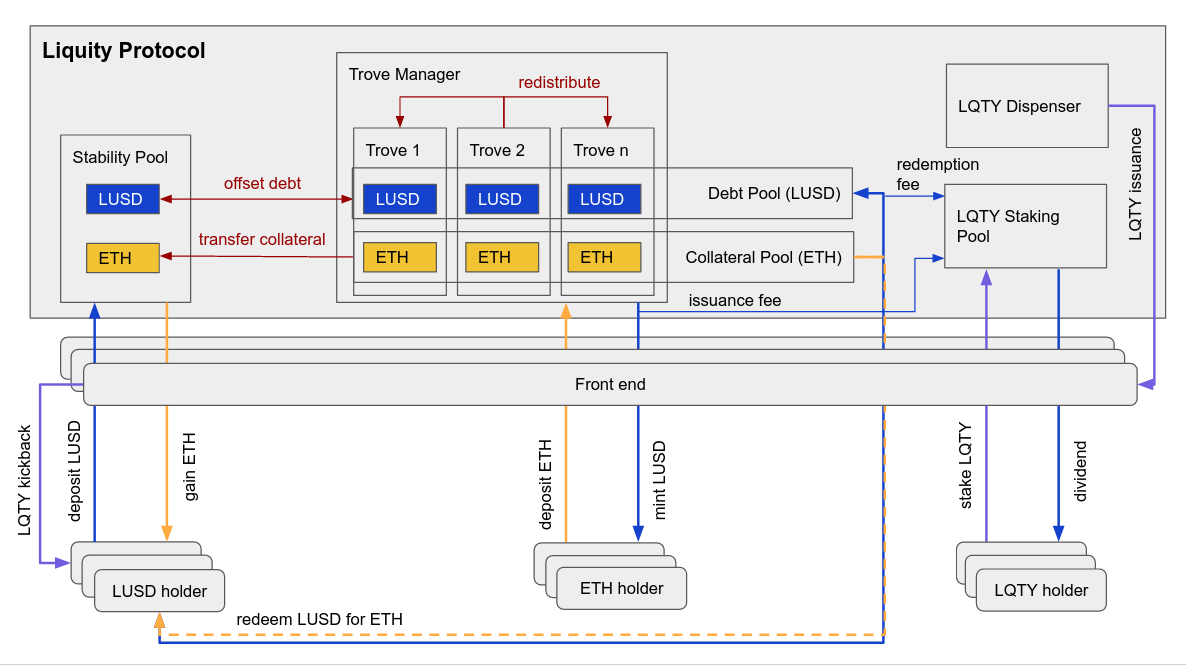
\includegraphics[width=16cm]{a14.png}
\end{figure}

We have thus introduced Liquity, a collateralized debt protocol with novel liquidation and redemption mechanisms that pushes the boundaries of capital efficiency and costs of liquidity. It is the first system of its kind that issues a stablecoin with a hard price floor against the underlying fiat currency. Furthermore, Liquity follows new paths to incentivize decentralization and growth from the start by tokenizing and redistributing a significant part of its protocol revenue to users and front end operators. 

\end{document}
